
\documentclass[fleqn,addpoints]{exam}
\usepackage{amsmath}
\usepackage{graphicx}
\usepackage{booktabs}
\usepackage{float}
\usepackage{caption}
\usepackage{polynom}
\usepackage{mdwlist}
\usepackage{cancel}

\usepackage{unitsdef} 
\newunit{\inch}{in}
\newunit{\mile}{mile}
\newunit{\mph}{mph}
\newunit{\foot}{ft}
\newunit{\knot}{knot}
\newunit{\gallon}{gallon}

\bracketedpoints
\everymath{\displaystyle}

\printanswers

\ifprintanswers 
\usepackage{2in1, lscape} 
\fi


% \begin{figure}[H]
%   \centering
%   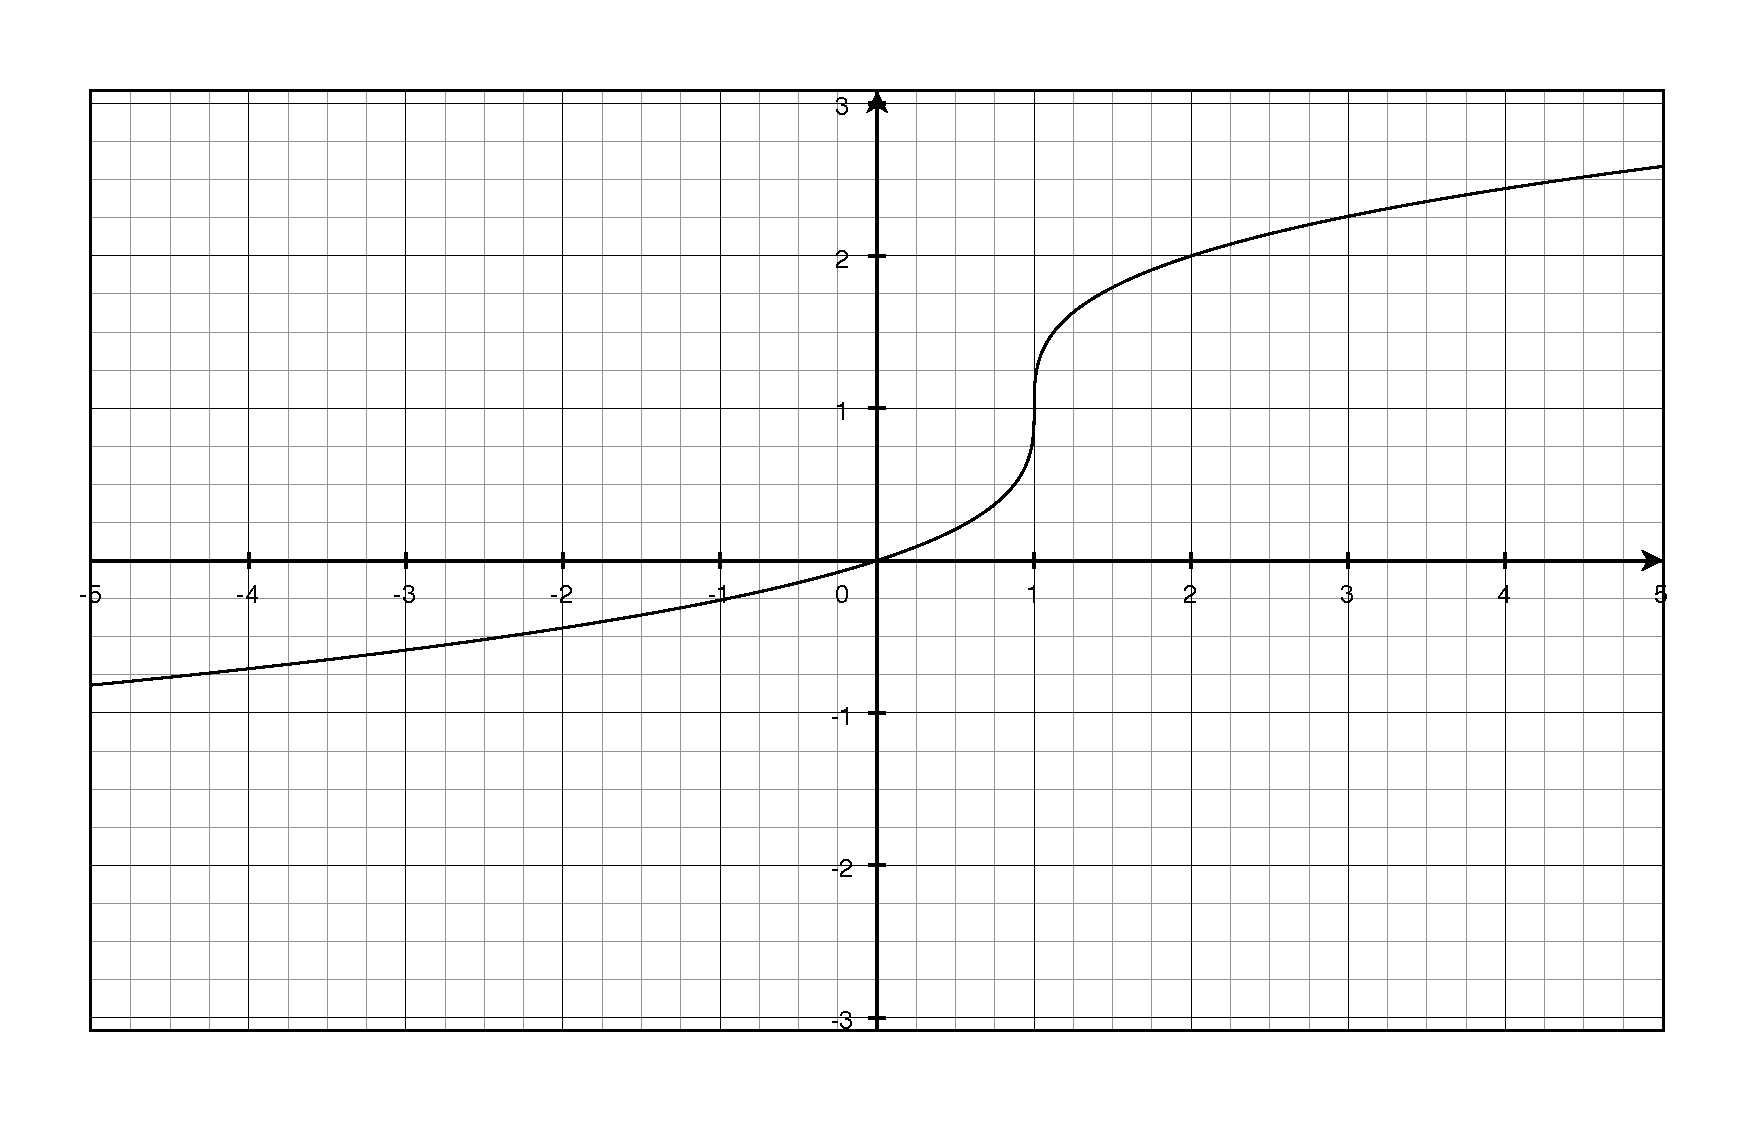
\includegraphics[scale=.3]{question7.eps}
%   \caption*{Question 7}
% \end{figure}

% \begin{tabular}{cc}
% \toprule
% period & amplitude \\
% \midrule
%   $\pi$ & $2$ \\
% \bottomrule
% \end{tabular}


%% \ifprintanswers
%% \usepackage{2in1, lscape}
%% \fi

\title{Math 263A Sample Final Two}
\date{October 25, 2012}

\author{}

\begin{document}

\maketitle  

\begin{questions}

\question Differentiate the function: $y = u (a \sec u + b \cot u)$.
\begin{solution}
If you don't remember the derivatives of secant and cotangent, you need to do a little preliminary work:
\begin{align*}
  D_x \sec x &= D_x (\cos x)^{-1} \\
  &= - (\cos x)^{-2} \cdot (- \sin x) \\
  &= \sec x \tan x \\
\\
  D_x \cot x &= D_x \frac{\cos x}{\sin x} \\
  &= \frac{\sin x \cdot (-\sin x) - \cos x \cdot \cos x}{\sin^2 x} \\
  &= - \frac{\sin^2 x + \cos^2 x}{\sin^2 x} \\
  &= - \frac{1}{\sin^2 x} \\
  &= - \csc^2 x \\
\end{align*}

Now we're ready to solve the problem:
\begin{align*}
  y &= u (a \sec u + b \cot u) \\
    &= au \sec u + bu \cot u \\  
\\
  y' &= a (u \sec u \tan u + \sec u) + b(u (- \csc^2 u) + \cot u) \\
     &= a (u \sec u \tan u + \sec u) + b(\cot u - u \csc^2 u) \\
\end{align*}
\end{solution}

\question Sketch the graph of a function $f$ for which:
\begin{itemize}
  \item $f(2) = 1$
  \item $\lim_{x \to 0^-} = 2$
  \item $\lim_{x \to 0^+} f(x) = -1$
  \item $\lim_{x \to 2^-} = 0$
  \item $\lim_{x \to 2+} f(x) = 1$
  \item $f(0)$ is undefined.
\end{itemize}

\begin{solution}
I can't get my computer to draw these graphs.
\end{solution}

\question Use the {\em Intermediate Value Theorem} to show that there is a root of the given equation in the specified
interval.  $x^4 + x - 3 = 0$, $(1, 2)$.

\begin{solution}
\begin{align*}
  f(1) &= -1 \\
  f(2) &= 15 \\
\end{align*}

Since $f(1)$ is negative and $f(2)$ is positive, the function must cross the x axis between $x = 1$ and $x = 2$, so the
function has a root in this interval.

\end{solution}

\question Find the derivative of the function using the definition of derivative. Also find the derivative of
the function using differentiation rules and compare. State the domain of the function and the domain of the derivative.
\[
  g(x) = \sqrt{1 + 2x}
\]

\begin{solution}

Using the definition of derivative:
\begin{align*}
  g'(x) &= \lim_{h \to 0} \frac{\sqrt{1 + 2(x + h)} - \sqrt{1 + 2x}}{h} \\
  &= \lim_{h \to 0} \frac{\sqrt{1 + 2x + 2h} - \sqrt{1 + 2x}}{h} 
      \cdot \frac{\sqrt{1 + 2x + 2h} + \sqrt{1 + 2x}}{\sqrt{1 + 2x + 2h} + \sqrt{1 + 2x}} \\
  &= \lim_{h \to 0} \frac{2 \cancel{h}}{\cancel{h} \left( \sqrt{1 + 2x + 2h} + \sqrt{1 + 2x} \right)} \\
  &= \lim_{h \to 0} \frac{2}{\sqrt{1 + 2x + 2h} + \sqrt{1 + 2x}} \\
  &= \frac{1}{\sqrt{1 + 2x}} \\
\end{align*}

Using the differentiation rules:
\begin{align*}
  g(x) &= (1 + 2x)^{1/2} \\  
  g'(x) &= \frac{1}{2} (1 + 2x)^{-1/2} \cdot 2 \\
        &= \frac{1}{\sqrt{1 + 2x}} \\
\end{align*}

The domain of $g$ is $\left[-\frac{1}{2}, \infty \right)$ and the domain of $g'$ is $\left( -\frac{1}{2}, \infty \right)$

\end{solution}

\ifprintanswers
\pagebreak
\fi

\question Find an equation of the tangent line to the curve at the given point: $y = (1 + 3x)^{20}$, $(0, 1)$.
\begin{solution}

Find the slope:
\begin{align*}
  y &= (1 + 3x)^{20} \\
  y' &= 60 (1 + 3x)^{19} \\
\\
  y'(0) &= 60 \\
\end{align*}
Find the equation:
\begin{align*}
  (y - 1) &= 60x \\
  y &= 60x + 1 \\
\end{align*}

\end{solution}

\question Find $\frac{dy}{dx}$ using implicit differentiation: $x^3 + x^2y + 4y^5 = 6$.
\begin{solution}

\begin{align*}
  x^3 + x^2y + 4y^5 &= 6 \\
  3x^2 + x^2y' + 2xy + 20y^4y' &= 0 \\
   x^2y' + 20y^4y' &= -3x^2 - 2xy \\
   % y'(x^2 + 20y^4) &= -3x^2 - 2xy \\
   y' &= \frac{-3x^2 - 2xy}{x^2 + 20y^4} \\
\end{align*}

\end{solution}

\ifprintanswers
\pagebreak
\fi

\question Use a linear approximation to estimate the number: $\sqrt{99.8}$.

\begin{solution}
  99.8 is very close to 100, so the answer will be 10 minus some small amount.  The problem is to find the small amount to subtract.

\begin{align*}
  y &= x^{1/2} \\
  dy &= \frac{1}{2} x^{-1/2} dx \\
     &= \frac{dx}{2 \sqrt{x}} \\
\\
  dy &= \frac{- 0.2}{2 \cdot 10} \\
     &= -0.01 \\
\\
  \sqrt{99.8} &= 10 - 0.01 = 9.99 \\
\end{align*}

\end{solution}

\question A right circular cylinder is inscribed in a cone with height $h$ and base radius $r$. Find the largest
possible volume of such a cylinder.

\begin{solution}
The first thing to do is to find the equation of the line that marks the border of the cone.  This is important because
it limits the height of the cylinder.

If the center of the cylinder is at the origin, the equation of the line is:
\[
  y = -\frac{h}{r} x + h
\]

If $x$ is the radius of the cylinder and $y$ is the height of the cylinder, the equation for the volume is:
\[
  V = \pi x^2y
\]
This is too many variables, but we can substitute the earlier expression for $y$ to get rid of $y$:
\begin{align*}
  V &= \pi x^2 \left( -\frac{h}{r} x + h \right) \\
    &= \pi \left( - \frac{x^3 h}{r} + x^2h \right) \\
\end{align*}

Differentiate and set $V$ equal to zero to find the maximum point:
\begin{align*}
  V'  &= \pi \left( -\frac{3x^2 h}{r} + 2xh \right) \\
\\
  \pi \left( - \frac{3x^2 h}{r} + 2xh \right) &= 0 \\
  x &= \left\{0, \frac{2r}{3} \right\} \\
\end{align*}

$x = 0$  definitely isn't a maximum, so the maximum is found at $x = \frac{2r}{3}$.  If you plug this number back in to the
equation for $y$, you find that $y = \frac{1}{3} h$.  This gives a total volume of $\frac{4 \pi r^2h}{27}$.

\end{solution}

\ifprintanswers
\pagebreak
\fi

\question If $y=x^3+2x$ and $\frac{dx}{dt} = 4$, find $\frac{dy}{dt}$ when $x=2$.
\begin{solution}
\begin{align*}
  y &= x^3 + 2x \\
  \frac{dy}{dt} &= 3x^2 \frac{dx}{dt} + 2 \frac{dx}{dt} \\
  &= (3x^2 + 2 )\frac{dx}{dt} \\
\\
  \frac{dy}{dt} &= (3 \cdot 4 + 2) \cdot 4 \\
    &= 56 \\
\end{align*}

\end{solution}

\question
Differentiate:
\[
  y = \sec^2 2x - \tan^2 2x
\]

\question
A particle moves on a vertical line so that its coordinate at time $t$ is $y = t^3 - 12t + 3$, $t \geq 0$.
\begin{parts}
\part Find the velocity and acceleration functions.
\begin{solution}
\begin{align*}
  y &= t^3 - 12t + 3 \\
  y' &= 3t^2 - 12 \\
  y'' &= 6t \\
\end{align*}
  
\end{solution}

\part When is the particle moving upward and when is it moving downward?
\begin{solution}
\begin{align*}
  3t^2 - 12 &= 0 \\
  t^2 - 4 &= 0 \\
  (t + 2)(t - 2) &= 0 \\
\end{align*}
The particle is moving down between $t = 0$ and $t = 2$ and up the rest of the time.  If time was allowed to be
negative, the particle was also moving down between $t = -2$ and $t = 0$, but the problem restricts the time to
non-negative numbers.

\end{solution}

\end{parts}

%% \question
%% Differentiate:
%% \[
%%   y = \sqrt[4]{\frac{x^2 + 1}{x^2 - 1}}
%% \]

\question
If a snowball melts so that its surface area decreases at a rate of $1 \centimeter^2 / \minute$, find the rate at which the
radius decreases when the radius is $5 \centimeter$.

\begin{solution}
\begin{align*}
  A &= \frac{4}{3} \pi r^2 \\
  \frac{dA}{dt} &= \frac{8}{3} \pi r \frac{dr}{dt} \\
  \frac{dr}{dt} &= \frac{3}{8 \pi r} \frac{dA}{dt} \\
\\
  \frac{dr}{dt} &= \frac{3}{40 \pi} \cm / \minute \\
\end{align*}

\end{solution}

\ifprintanswers
\pagebreak
\fi

\question $f(x) = \frac{1}{x^2 - 9}$
\begin{parts}
\part Find the derivative of the function.
\begin{solution}
\begin{align*}
  f(x) &= (x^2 - 9)^{-1} \\
  f'(x) &= -(x^2 - 9)^{-2} \cdot 2x \\
       &= \frac{-2x}{x^2 - 9}
\end{align*}
\end{solution}

\part Find the vertical and horizontal asymptotes.
\begin{solution}
Since the degree of the numerator is less than the degree of the denominator, there is a horizontal asymptote 
at $y = 0$.

The denominator is 0 when $x = \pm 3$, so there are vertical asymptotes at $x = \pm 3$.

\end{solution}

\part Find the intervals on which $f$ is increasing or decreasing. 
\begin{solution}
The critical points are the two vertical asymptotes and the point where $f'(x) = 0$.  These are: $x = \{-3, 0, 3\}$.  If
you check some sample points or do a sign chart, you can see that:
\begin{itemize*}
\item $f$ is increasing on $(-\infty, -3) \cup (-3, 0)$
\item $f$ is decreasing on $(0, 3) \cup (3, \infty)$
\end{itemize*}
\end{solution}

\ifprintanswers
\pagebreak
\fi

\part Use the information from (a)-(d) to sketch the graph.
\begin{solution}
\begin{figure}[H]
  \centering
  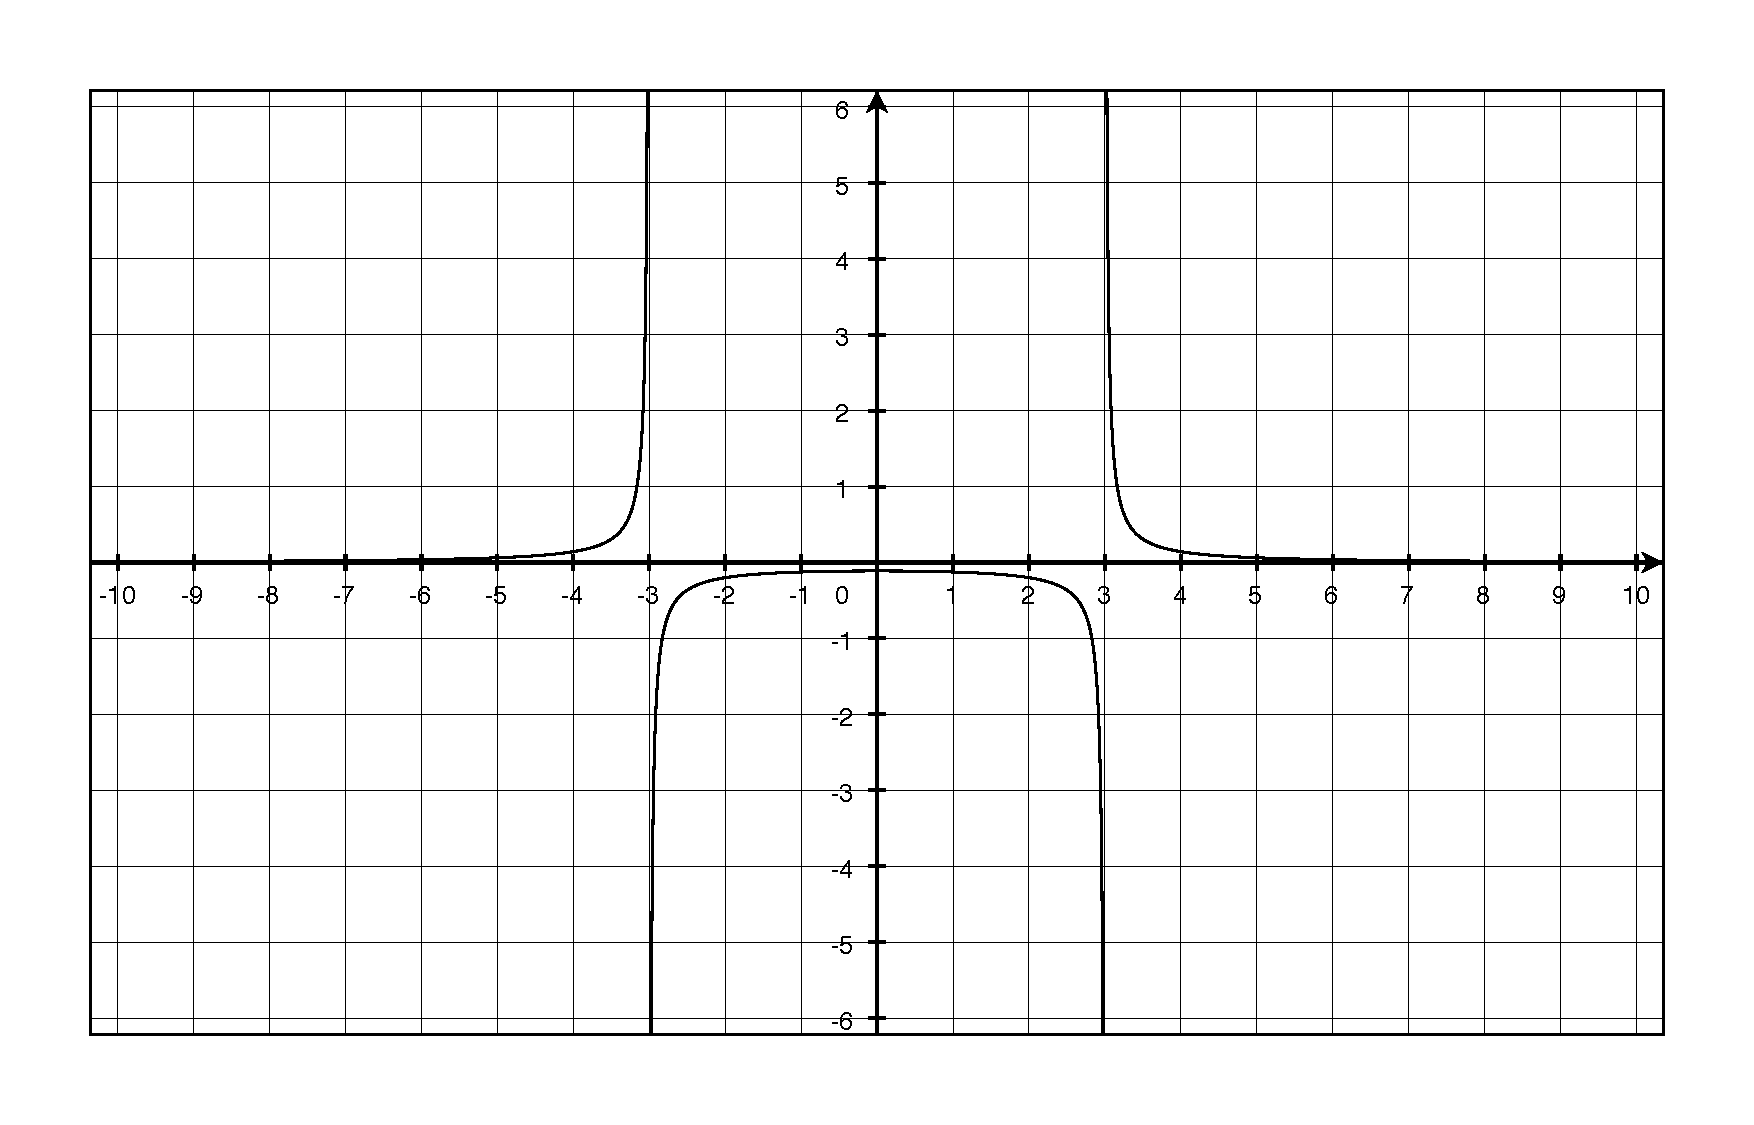
\includegraphics[scale=.3]{final_2_q13.eps}
  \caption*{Question 13}
\end{figure}
\end{solution}

\end{parts}

%% \question $f(x) = x - 2 \sin x$, $0 < x \leq 3π$

%% \begin{parts}
%% \part Find the intervals on which $f$ is increasing or decreasing. 
%% \begin{solution}
%% \begin{align*}
%%   f(x) &= x - 2 \sin x \\
%%   f'(x) &= 1 - 2 \cos x \\
%% \\
%%   1 - 2 \cos x &= 0 \\
%%   \cos x &= \frac{1}{2} \\
%%   x &= \left\{ \frac{\pi}{3}, \frac{5 \pi}{3}, \frac{7 \pi}{3},  \right\}
%% \end{align*}

%% $x$ is increasing on $\left( \frac{\pi}{3}, \frac{5 \pi}{3} \right) \cup \left( \frac{7 \pi}{3}, 3 \pi \right)$ and decreasing on
%% $\left( \frac{5 \pi}{3}, \frac{7 \pi}{3} \right)$

%% \end{solution}

%% \part Find the local maximum and minimum values of $f$.
%% \begin{solution}
%% \end{solution}

%% \part Find the intervals of concavity and the inflection points.
%% \part Sketch the graph of the function.
%% \end{parts}

\end{questions}

\end{document}
